\chapter{Литературный обзор} \label{chapt1}

Для того чтобы отслеживать активность любого объекта, можно представить что в каждый момент времени у этого объекта существует состояние. На шкале времени состояние объекта может меняться, таким образом мы поймём что объект был неподвижен или наоборот, совершал активность - в нашем случае смену состояния.

Состояние объекта можно описать непрерывными функциями - как, например, координаты тела в пространстве. А можно дискретными, когда количество состояний ограничено. Пример - человек смотрит в камеру, в сторону, вверх.

% два изображения: машина на координатной оси, человек на 2 кадрах расположен анфас, в профиль

Для отслеживания базовой активности собак, нам подойдут оба эти варианта. Возможно отслеживать как координаты каждой конечности собаки - лап, хвоста, туловища, головы. Такая задача в иностранной литературе будет называться Pose Estimation и подразумевает возвращение некоторой функцией координат тела в двумерном пространстве кадра и 3D Pose Estimation, если требуется получить вектор перемещения и поворота относительно камеры. 

% картинка с Pose estimation и 3D pose estimation
\begin{figure}[ht] 
  \center
  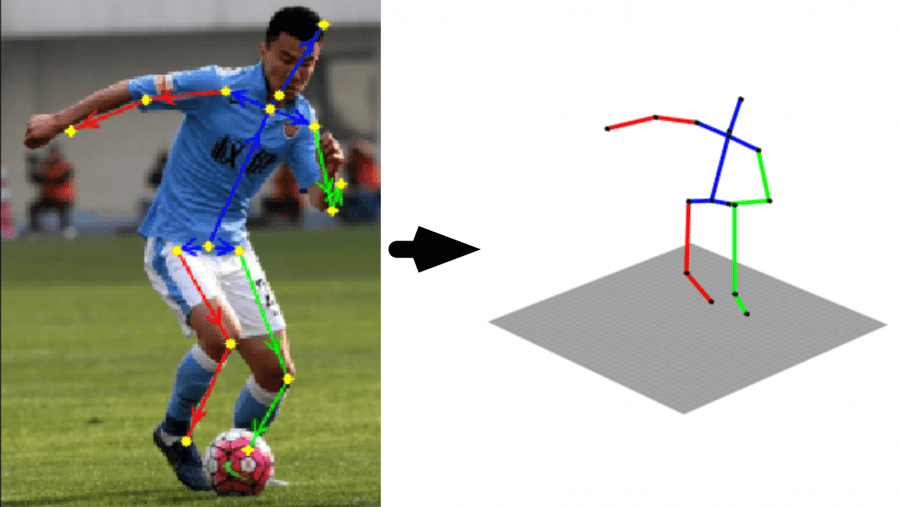
\includegraphics [scale=0.33] {3dposeest}
  \caption{3D Pose Estimation} 
  \label{img:3dposeest}  
\end{figure}


Так как конечная цель работы - классифицировать простые активности собаки, например, когда собака сидит, стоит или лежит - задачу Pose Estimation решать необязательно, но она может значительно упростить дальнейшую классификацию, так как позволить отбросить избыточную визуальную информацию, которую мы получаем на фотографии.



\section{Существующие датасеты} \label{sect1_1}
Насколько известно автору, по состоянию на Май 2020 года в открытом доступе содержатся только следующие наборы данных с изображениями собак:
\begin{enumerate}
  \item ImageNet \cite{imagenet} - Считается крупнейшим датасетом по классификации всего. Насчитывает более 1 миллиона изображений и больше 1000 классов изображений для классификации, начиная от машин, заканчивая собаками. Часто используется для оценки производительности систем компьютерного зрения а также для предобучения нейронных сетей при недостаточных данных.
  \item Stanford Dog Dataset \cite{KhoslaYaoJayadevaprakashFeiFei_FGVC2011} - Подраздел ImageNet. В нём содержится 20000 изображений собак 120 различных пород. Разметка осуществлялась для дальнейшей классификации собак по породам. Разные породы имеют различное количество изображений.
  \item OpenImageDataset \cite{openimages} - ближайший аналог ImageNet по назначению и реализацию, за тем лишь исключением что он создавался с уклоном в детекцию объектов, поэтому все изображения там чуть большего размера, и на каждом изображения может быть несколько объектов, в том числе, разного класса. К каждому объекту прилагается информация о его ограничивающей рамке.
  \item DogCentric Activity Dataset \cite{yumi2014first} - Датасет с видеозаписями различных занятий собаки от лица самой собаки. Целью является классификация активности.
  \item Jena Action Recognition Dataset \cite{jena} - Коллекция видеозаписей с дистанционно управляемым роботом-собакой SONY ERS-7 Aibo. Создавалась для оценивания систем распозанавания. В ней есть видеозаписи, координаты ограничивающих рамок робота на каждом кадре и данные для калибровки.
\end{enumerate}
Все эти датасеты достаточно хорошо размечены. Важно заметить что в изображения собак в ImageNet, Stanford Dog Dataset и OpenImageDataset пересекаются, так что суммарно по этим трём датасетам имеется всего 20000 изображений собак, столько же сколько и в Stanford Dog Dataset.

\section{Методы решения задачи} \label{sect1_2}
В области определения позы животных проделано сильно меньше работы, чем в этой же области для людей. Причины очевидны:
\begin{itemize}
    \item Широкая возможность применения
    \item Возможность использовать актёров
    \item Большое количество фотографий
\end{itemize}
\subsection{На людях} \label{subsect1_2_1}
Сейчас классификацию позы людей осуществляют с помощью так называемого Pose Estimation Tree. Целью зрения становится будто восстановить человеческий скелет по изображению. Для этого определяются важные повижные узлы - joints. Обычно ими являются локти, колени и другие суставы. У человека всего порядка 200 таких узлов. При этом при решении большинства задач компьютерного зрения используется около 20.
\begin{figure}[ht] 
  \center
  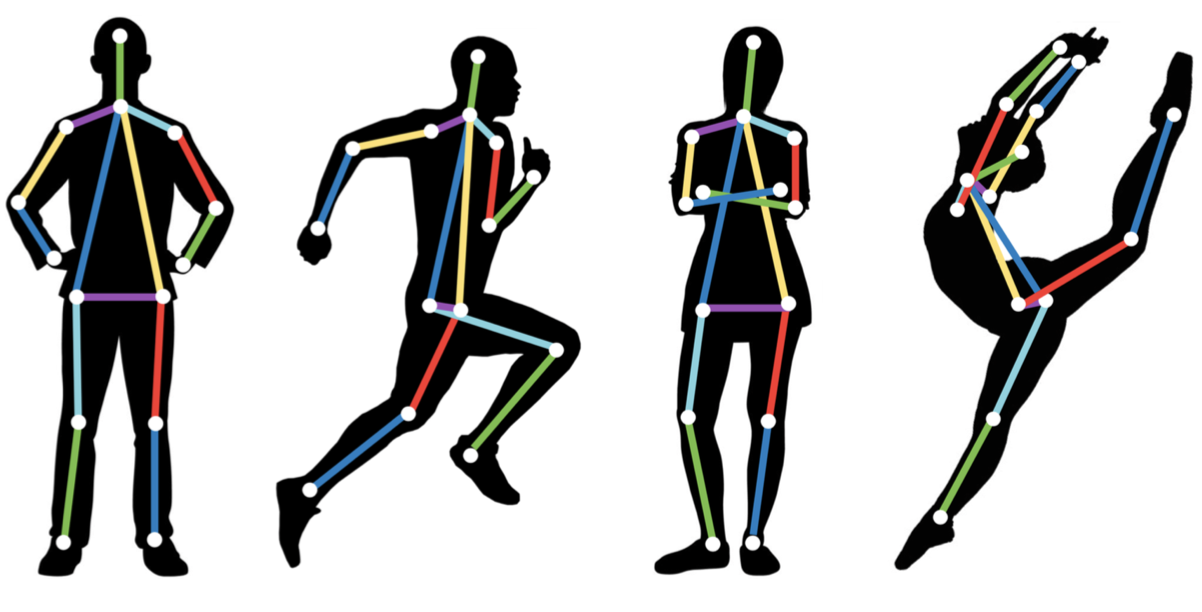
\includegraphics [scale=0.33] {pose}
  \caption{Pose Estimation Tree} 
  \label{img:poseest}  
\end{figure}

Классические пакетные решения для такой задачи - Tensorflow Pose Kit и OpenPose. Всё что требуется для этих пакетов - набор размеченных данных для обучения. OpenPose может работать с множественными объектами и окклюзиями, но относительно медленный. Tensorflow Pose Kit создан с уклоном в перенос модели на портативные устройства.

\subsection{На животных} \label{subsect1_2_2}
В 2018 году вышла публикация \cite{deeplabcut}, в которой авторы предложили новаторский способ автоматически следить за указаными частями тела у животных. Алгоритму не требуется больших датасетов с данными, нужно всего около 200 кадров (от 8 секунд видео) чтобы предсказать остальной видеопоток. 
\begin{figure}[ht] 
  \center
  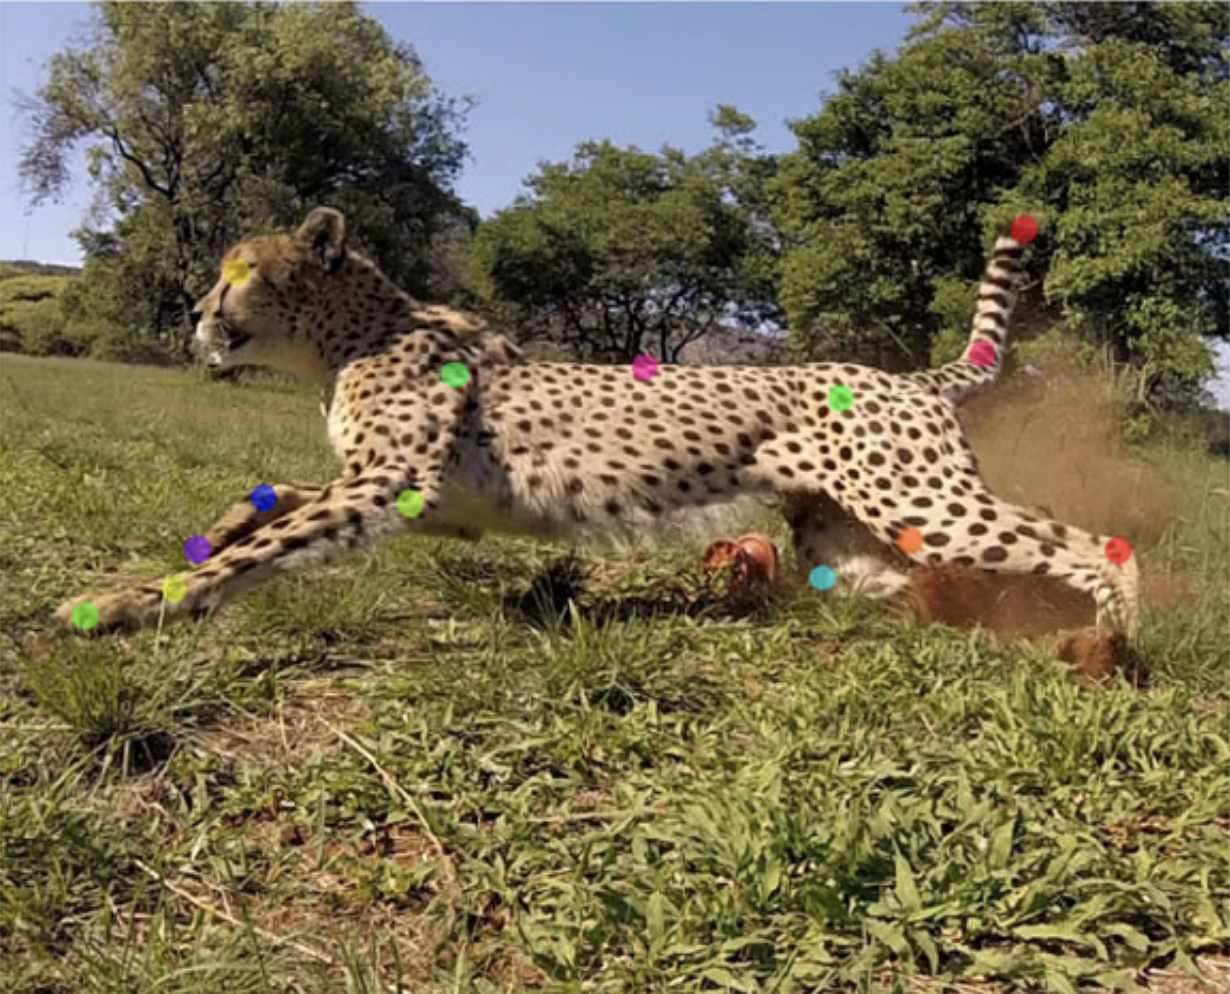
\includegraphics [scale=0.33] {deeplabcut}
  \caption{Предсказанный кадр DeepLabCut} 
  \label{img:deeplabcut}  
\end{figure}
Ограничениями данного метода являются необходимость в разметке этих первых 200 кадров, на это уходит обычно около 20 минут, а также принципиальная возможность работать только с видеопотоком. 
В итоге это достаточно хороший метод для того чтобы разметить большие видеопотоки. Алгоритм обеспечивает достаточную точность и на длинных видеозаписях позволяет сильно сократить время на разметку данных для Pose Tree Estimation. Применение данного способа не ограничивается только на животных: любой видеопоток, на котором можно отслеживать объекты будет работать.

\section{Разметка данных} \label{sect1_3}
Обязательным процессом любой задачи связанной с машинным обучением является получение и разметка данных. Разметкой данных в зависимости от объёма можно заниматься как самостоятельно, так и с помощью наёмного труда. 

\subsection{Самостоятельная разметка данных} \label{subsect1_3_1}
Нет ничего страшного в том чтобы разметить несколько тысяч изображений. Практика показывает, что на самостоятельную разметку тысячи изображений при наличии необходимых инструментов уходит от 20 минут до часа.

К достоинствам самостоятельной разметки можно отнести:
\begin{itemize}
    \item Надёжность - возможность полностью контролировать результат
    \item Независимость - нет нужды полагаться на других людей или сервисы
    \item Дешевизна - не нужно никому платить
    \item Возможность ознакомится с набором данных
\end{itemize}
И действительно, ознакомившись с набором данных, можно увидеть его недостатки, или наоборот, особенности, которые могут помочь решить задачу.
Недостатки:
\begin{itemize}
    \item Разметка больших наборов данных изнуряет
    \item Это самый медленный способ получить данные
    \item Часто приходится создавать инструменты для разметки самостоятельно
\end{itemize}


\subsection{Разметка данных с помощью сторонних сервисов} \label{subsect1_3_2}
Когда самостоятельная разметка невозможна или занимает слишком много времени, можно воспользоваться специальными сервисами для разметки данных. Такими являются Яндекс.Толока и Amazon Mechanical Turk.

Достоинства:
\begin{itemize}
    \item Скорость - из-за большого количества пользователей на разметку даже больших датасетов редко уходит больше часа.
    \item Встроенные в сервисы инструменты для разметки
    \item Относительная дешевизна.
\end{itemize}
Недостатки:
\begin{itemize}
    \item Качество разметки крайне низкое
    \item Для сложных заданий требуется составлять обучение
    \item Требуется опыт в составлении заданий на платформе
    \item Невозможность разметки коммерчески секретных данных
\end{itemize}
Главным недостатком таких сервисов является то, что пользователи не знают ничего о задаче автора. Поэтому задания надо составлять максимально точно, и заставлять пользователей проходить обучение прежде чем решать задачу. Более того, часть пользователей могут вместо правильных ответов давать быстрые, и за этим тоже необходимо следить.

\subsection{Разметка данных с помощью наёмного штата} \label{subsect1_3_3}
Обычно, серьёзные команды на рынке машинного обучения для разметки данных используют собственные наёмные команды.

Достоинства:
\begin{itemize}
    \item Высокое качество разметки
    \item Возможность получать обратную связь
    \item Возможность лично и устно формулировать задания штату
    \item Возможность подписать соглашение о неразглашении
\end{itemize}
Недостатки:
\begin{itemize}
    \item Цена. Это самый дорогой способ
\end{itemize}
Часто такие команды нанимают под однотипные задачи. Например, если есть постоянный поток данных с камер автомобилей, такая команда может размечать данные специально для компании. В таком случае можно обеспечить постоянную нагрузку на штат, а сотрудники будут опытными в решении задачи.